\section{Evaluation}
\label{sec:eval}

In this section, we first evaluate our algorithm by 
varying $k$ and test the overlap between concepts.
We then demonstrate the effectiveness of the generated 
action concepts by applying them to two applications: 
verb similarity and verb clustering.
%building small lexicons of
%just 20 randomly selected English verbs (our development set)
%by varying parameter $k$ and testing the quality
%of these lexicons.
%We then construct two large lexicons of 10,116 verbs using the
%parameters tuned from previous small lexicons.
%We show the key characteristics of these lexicons and the time cost
%for constructing them.
%We then demonstrate the effectiveness of these comprehensive lexicons
%by applying them to several applications: verb sense matching,
%argument identification, word sense disambiguation,
%action frame generation and term similarity.
%an action concept lexicon for 3734 English
%verbs, evaluate its quality and show the effective of
%our lexicon on several applications.
%We present the datasets and preprocessing.
%Then, we evaluate the accuracy and overlap of the lexicon built.
%We further show the parameter tuning
%and report the execution times of the AC algorithm.
%After that, we evaluate the action concept's ability to
%identify different senses of verbs by matching
%the action concepts to WordNet synsets.

\subsection{Experimental Setup}
\label{sec:preprocess}
In this paper, we use Probase\cite{WuLWZ12} and WordNet\cite{wordnet}
as two alternative isA taxonomies. Probase is a large collection of
concept-subconcept or concept-entity pairs which were
extracted automatically by the Hearst pattern\cite{Hearst92} from
a large web corpus. Because this knowledge base is harnessed from large
data, it contains statistical scores of the extracted pairs,
such as the popularity,
and the conditional probability between the concept and its sub-concept.
WordNet, on the other hand, is a smaller, cleaner knowledge base manually
curated by experts and does not contain any scoring information.
These two taxonomies provide two different vocabularies of concepts
from which to draw the solution of AC.
%Our primary target of verb is a set of 200 most frequently used verbs in
%English text\footnote{We compute the frequency of all verbs that appeared
%in a very large web text corpus to obtain the 200 most frequently used
%verbs. We excluded a few verbs such as ``use'', ``make'', ``get'' and
%``take'' from the top of the list because they are extremely general and
%have too many arguments.},
%which we call Verb-200. These verbs are shown in \figref{fig:verbs}. A random
%sample of 20 verbs from Verb-200 forms a smaller set of verbs called Verb-20
%(highlighted in \figref{fig:verbs}) which are used in most of our experiments.

All our experiments are based on two large
datasets\footnote{We release most of
our datasets and the action concept lexicon at
\url{http://adapt.seiee.sjtu.edu.cn/~kzhu/ac}.}
from Web sentences (called Web for short) and
Google syntactic N-gram data\cite{goldberg2013,googlengram}
(called Google for short), respectively.
The 3734 most frequently used verbs (including verb phrases)
in the Web data form a primary verb set called {\bf Verb-3734}.
A subset of 2323 verbs that can be found in the Google dataset
form another verb set called {\bf Verb-2323}.
%We compute the frequency of all verbs that appeared
%in a very large web text corpus to obtain the 3734 most frequently used
%verbs.
A random sample of 20 verbs from the 200 most frequently
used verbs form the smallest set of verbs called {\bf Verb-20}
(in \figref{fig:verb20}), %which are used in most of our experiments.
which are used in some of the experiments.

The Web dataset contains 49,911,718 verb-subject pairs
and 65,035,827 verb-object pairs extracted from 165,758,215 English
sentences, which is a crawled snapshot of web pages.
%\KZ{How many subject-verb pairs and verb-object pairs in web data?}
%\KZ{How many?}\textcolor{red}{[KQ:We don't know...]}
%in a snapshot of Bing's search log.
The Google dataset contains
32,731,395 verb-subject pairs and 43,580,062 verb-object pairs
from the \emph{Verbargs} package, which includes 130,436,458
syntactic N-grams.% with verb-argument dependencies.
%\KZ{How many subject-verb pairs and verb-object pairs in google data?}
%\KZ{Kaiqi: We need to describe how we generate the web and
%google data sets here.
%Need to emphasize how big these data sets. Remember this ``VL''DB!}

\begin{figure}[th]
\centering
\fbox{\parbox{.8\columnwidth}{
bring,
carry,
connect,
cut,
define,
eat,
help,
hit,
keep,
operate,
perform,
play,
read,
release,
report,
select,
spend,
submit,
visit,
wear
}}
\caption{Verbs in Verb-20}
\label{fig:verb20}
\end{figure}

ReVerb also provides millions of relation triples, some of which contain
verbs as predicate.
%However, the scale of ReVerb is small to our problem.
We aim at discovering the action concepts,
which needs a large number of action instances
for each verb. However, ReVerb contains small number of triples for each verb.
For example, only 374 unique triples for ``wear'' are
extracted in ReVerb while our web dataset contains 17,749 unique
\pair{verb}{object} pairs for ``wear''.
The reason of the huge different is that,
a triple must contain two arguments for the verb in ReVerb. However,
verbs co-occur with only one argument in many cases.
Moreover, ReVerb has little coverage on
intransitive verbs, which only come with subject.
We give up using ReVerb data due to these limitations.
%\KZ{We need to explain why we don't use the ReVerb data.}

%\subsection{Preprocessing of Dataset}
%To make use of the web sentences and Google syntactic N-gram,
Next, we preprocess the two datasets as follows to
generate action instances.

{\bf Web} data comes from the result of Stanford dependency parser,
%We run a dependency parser on the whole corpus and
which are dependency trees for the sentences. We are interested in
verb-subject and verb-object relations only.
The head word of subject is usually labeled
as ``nsubj'' or ``agent'' while the head word of object is usually
labeled as ``dobj'' or ``nsubjpass''.
We can retrieve the entire phrase of subject or object in the dependency
tree by returning the whole subtree rooted on the head.
However, the whole phrase of subject/object is not always
a term recognizable by the taxonomies. As shown in \figref{fig:pterm},
the phrase ``a flashy baseball cap''
is extracted as the object of ``wear'', but 
it is not a valid Probase/WordNet term.
To make use of the taxonomies, we need to
detect the Probase/WordNet term from the subject/object phrase
(e.g., baseball cap).

\begin{figure}[th]
\centering
\epsfig{file=pterm.eps,width=0.8\columnwidth}
\caption{Dependency Parse Tree}
\label{fig:pterm}
\end{figure}

We use a sliding window strategy to extract longest
Probase/WordNet term that we can detect in the whole phrase.
The window slides around the head word
from right to left, and check if a Probase/WordNet term exists.
The initial size of the window is the length of the
whole phrase. If we detect a Probase/WordNet term,
we return the phrase captured in the window;
Otherwise, we decrease the window size and slides
around the head term again. We stop until we find
any Probase/WordNet term. Usually, this procedure can detect
a Probase/WordNet term from the phrase, because Probase/WordNet includes
most of the words (phrase with length 1). After
preprocessing, we output all the pairs of verb-subject and
verb-object as action instances.
%\begin{table}[th]
%\centering
%%\scriptsize
%\caption{Snapshot of Google Syntactic N-gram}
%\begin{tabular}{|l|l|}
%\hline
%Verb & N-gram \\
%\hline \hline
%accept & firms/NNS/nsubj/2\; accept/VBP/conj/0\; \\
%& money/NN/dobj/2\; in/IN/prep/2\; \\
%& exchange/NN/pobj/4   \\
%\hline
%delay & to/TO/aux/2\; delay/VB/xcomp/0\; \\
%& these/DT/det/4\; matters/NNS/dobj/2 \\
%\hline
%spent & an/DT/det/2\; afternoon/NN/nsubjpass/4\; \\
%& was/VBD/aux/4\; spent/VBN/conj/0\\
%\hline
%\end{tabular}
%\label{tab:ngram}
%\end{table}

\textbf{Google} data contains relations between
verbs and arguments.
%A snapshot
%of Google syntactic n-gram is shown in \tabref{tab:ngram}.
%The syntactic n-gram consist of the dependency parsing
%result conducted by Stanford parser.
Each token is labeled with POS tag, dependency and head index.
To apply this data to our task,
we restore each n-gram to a dependency tree according
to the head index and 
adopt the same processing as in Web to extract 
pairs of \pair{verb}{subject} and \pair{verb}{object}.
%First, we restore each n-gram to a dependency tree
%according to the head index. Next, we find the head of the
%subject or object from the nodes that directly connects to
%the verb node with a dependency label such as ``nsubj'', ``agent'', ``dobj''
%or ``nsubjpass''. Around the head, we use the same sliding window
%algorithm to find a longest Probase/WordNet term to be the subject/object
%as in the processing of the web data. Also, we convert
%the verb to its lemma form.
%After this process, we finally get two lists of pairs
%in the form of \pair{verb}{subject} and \pair{verb}{object}, respectively.

The subsequent experiments are conducted on lexicons learned from
different combinations of verb sets, taxonomies and datasets. For
readers' convenience, the configurations of these experiments are documented
in \tabref{tab:comb}.
\begin{table}[th]
\centering
%\scriptsize
\caption{Verbs, taxonomies and datasets for each experiment}
\begin{tabular}{|l|c|c|c|}
\hline
Experiment & Verb Sets & Taxonomies & Datasets \\
\hline \hline
Accuracy \& Overlap & Verb-20 & Probase &  Web, Google\\
\hline
\multirow{2}{*}{Execution Times} & Verb-3734, & Probase,
	& \multirow{2}{*}{Web, Google} \\
	& Verb-2323 & WordNet & \\
\hline
Verb Sense Matching & Verb-3734 & WordNet & Web \\
\hline
Argument Identification & Verb-20 & Probase & Web \\
\hline
WSD & Verb-3734 & WordNet & Web \\
\hline
Verb Frame Generation & Verb-3734 & Probase & Web \\
\hline
Term Similarity & Verb-3734 & Probase & Web \\
\hline
\end{tabular}
\label{tab:comb}
\end{table}

%\begin{figure}[th]
%\centering
%\fbox{\parbox{2\columnwidth}{
%\sout{use
%make
%include
%take
%get
%provide
%show}
%go
%say
%find
%see
%come
%work
%need
%look
%require
%give
%{\bf help}
%offer
%know
%create
%change
%add
%start
%allow
%{\bf keep}
%{\bf play}
%contain
%run
%apply
%receive
%call
%develop
%leave
%begin
%hold
%support
%cause
%build
%meet
%increase
%cover
%base
%want
%serve
%continue
%{\bf read}
%write
%produce
%{\bf bring}
%involve
%pay
%live
%ask
%put
%consider
%set
%reduce
%remove
%improve
%appear
%{\bf perform}
%seem
%move
%lead
%follow
%buy
%occur
%try
%design
%contact
%complete
%sell
%learn
%determine
%think
%{\bf report}
%describe
%like
%present
%mean
%relate
%lose
%feel
%affect
%post
%represent
%enjoy
%send
%open
%discuss
%{\bf visit}
%enter
%grow
%share
%maintain
%identify
%indicate
%tell
%place
%list
%return
%choose
%{\bf select}
%turn
%sign-up
%form
%obtain
%stop
%check
%result
%win
%happen
%install
%{\bf wear}
%die
%love
%understand
%save
%expect
%focus
%fill
%watch
%prevent
%{\bf spend}
%protect
%reach
%pass
%raise
%display
%treat
%ensure
%{\bf connect}
%achieve
%establish
%suggest
%view
%accept
%associate
%fit
%drive
%exist
%control
%talk
%replace
%deliver
%avoid
%hear
%fall
%let
%{\bf define}
%handle
%{\bf eat}
%plan
%bear
%prepare
%manage
%{\bf release}
%promote
%attend
%experience
%join
%kill
%seek
%{\bf operate}
%measure
%end
%refer
%teach
%face
%conduct
%explain
%purchase
%combine
%test
%{\bf cut}
%generate
%review
%deal
%break
%close
%reflect
%decide
%believe
%consist
%{\bf carry}
%fail
%collect
%speak
%address
%encourage
%match
%stand
%sit
%stay
%{\bf hit}
%{\bf submit}
%draw
%walk
%depend
%limit
%please
%reveal
%introduce
%wait
%arrive
%enable
%}}
%\caption{Verb-200 (Ranked) with Verb-20 in Bold}
%\label{fig:verbs}
%\end{figure}

%bring\\
%carry\\
%connect\\
%cut\\
%define\\
%eat\\
%help\\
%hit\\
%keep\\
%operate\\
%perform\\
%play\\
%read\\
%release\\
%report\\
%select\\
%spend\\
%submit\\
%visit\\
%wear\\
%\hline
%\end{tabular}
%\label{tab:verbs}
%\end{table}
%



\subsection{Accuracy (P-R) and Overlap (vs. SP)}
\label{sec:accuracy}
We run AC algorithm on Web and Google datasets,
using either MI or TF-IDF as the confidence function to obtain
action concept lexicon for $k=1 \dots 10$, 
and for both subjects and objects of all verbs in
Verb-20. We set the parameter $\tau=0.2$, which will be discussed
in \ref{sec:decision_tau}.
%As an example, \tabref{tab:top5result} shows the
%top 5 object concepts for Verb-20 extracted using MI on Web data.
In this section, we show the accuracy of the action concepts
and the degree of their overlaps for each verb in Verb-20.
Our baseline is the top $k$ concepts learned by
selectional preference (SP)\cite{resnik1996selectional}.
SP computes the selectional association between a semantic class $c$
and a predicate $p$ as:
\begin{equation}
A(p,c)=\frac{Pr(c|p)\log\frac{Pr(c|p)}{Pr(c)}}
{\sum_{c'\in C}{Pr(c'|p)\log\frac{Pr(c'|p)}{Pr(c')}}},
\end{equation}
where $C$ is the collection of semantic classes.
%This score measures the difference between the prior probability
%$p(c)$ and posterior distribution
%$p(c|p)$. A large difference stands for high co-occurrence of $c$ and $v$,
%and hence the class and the verb are strongly coupled.

%Since we mainly focus on evaluating the object concepts extracted by
%our approaches, we abuse using the term \emph{argument}
%to refer to object of the verbs in the following experiments.
%\begin{table}[th]
%\caption{Top 5 Object Concepts Extracted by AC on the Web Data}
%\center
%\small
%% Table generated by Excel2LaTeX from sheet 'Sheet1'
%\begin{tabular}{|l|l|}
%    \hline
%    Verb  & Object Concepts\\
%    \hline \hline
%    bring	&person,issue,item,material,factor\\
%    \hline
%    carry	&weapon,product,name,species,factor\\
%    \hline
%    connect	&device,system,component,area,technology\\
%    \hline
%    cut	&material,part,factor,accessory,issue\\
%    \hline
%    define	&group,event,feature,factor,document\\
%    \hline
%    eat	&food,plant,dish,ingredient,flavor\\
%    \hline
%    help    &person,community,company,organization,group\\
%    \hline
%    hit	&place,feature,artist,application,item\\
%    \hline
%    keep	&information,name,item,area,feature\\
%    \hline
%    operate	&system,facility,service,device,technology\\
%    \hline
%    perform	&task,procedure,service,activity,method\\
%    \hline
%    play    &game,character,player,activity,name\\
%    \hline
%    read	&book,information,newspaper,site,classic\\
%    \hline
%    release	&information,name,product,material,player\\
%    \hline
%    report	&crime,event,infection,species,organization\\
%    \hline
%    select	&item,name,topic,feature,company\\
%    \hline
%    spend	&time,money,fund,occasion,festival\\
%    \hline
%    submit	&information,document,datum,documentation,material\\
%    \hline
%    visit	&site,place,community,attraction,name\\
%    \hline
%    wear	&clothing,item,style,accessory,device\\
%    \hline
%    \end{tabular}%
%\label{tab:top5result}
%\end{table}


\subsubsection{Accuracy}
We use precision, recall and $F_1$ measure to evaluate our
algorithm and the generated lexicon.

\textbf{Precision}:
%We use precision to evaluate the quality of concepts produced by each
%algorithm.
For a given verb, a good concept for an argument type
(subject or object) not only covers as many as arguments in the dataset,
but also contains few entities that are invalid for that verb.
The precision score for each verb is:
\[
Precision = \frac{\sum_{c \in C_k}|E_c|\times Precision(c)}
{\sum_{c \in C_k}{|E_c|}},
\]
\[
Precision(c)=\frac{|\mbox{Entities in~} c
\mbox{~which are correct arguments}|}{|E_c|}.
\]
%where $|E_c|$ is the number of entities in concept $c$ and
%$C_k$ is the set of 10 argument concepts discovered by the algorithms.
%We build a ground truth dataset for Verb-20 by
Annotating all entities for each concept needs a large
amount of human efforts. We use a sample strategy to
estimate $Precision(c)$ for a concept $c$. Specifically,
we sample 10 entities from each of the $k$ argument concepts
for each verb learned by the AC and SP.
%discovered by the algorithm.
%To make more typical entities to be more easily sampled out,
%the sampling is conducted according to the typicality of the entities.
%The resulting annotation set comprises 2000 unique entities.
Each entity is then labeled whether it is a correct argument to the
verb by majority of three human judges.
We compare the our algorithm, i.e., AC(MI) and AC(TF-IDF) to
SP in terms of precision on both Web and Google.
The overall precision of the 20 verbs
is reported in \figref{fig:precision_web} and \figref{fig:precision_ngram}.
%For all the algorithms, we keep the top-k concepts for the argument of
%each verb.
For the Web data, as the number of concepts $k$ grows, the precision generally
decreases in all methods. For the Google data, the precision is relatively
stable across different values of $k$.
%This phenomenon indicates that the smaller scale of
%the data causes smaller disparity of the overall quality for different size of concepts we get.
In both datasets, AC(MI) outperforms AC(TF-IDF) and
SP by significant margins. AC(TF-IDF) gives low precision,
perhaps because the TF-IDF scoring doesn't penalize the incorrect arguments
sufficiently but instead prefers to select more general
concepts to maximize the score (\eqnref{eq:approxf}).
%The greedy solution loses in terms of precision
%comparing to local search and selectional preference because it prefers
%to select general concepts to minimize the number of concepts.
%Simulated annealing is able to jump out of the local optimal and
%find a solution that close to the global optimal.
%The comparison among the three approaches on web sentence dataset
%shows that our local search algorithm is enable to find concepts
%with proper granularity, i.e., covering most correct arguments but
%less incorrect arguments. We also compare the precision of
%applying local search to web sentence data with that to Google
%syntactic N-grams.

\textbf{Recall}: Recall measures the coverage of
correct arguments of a verb by the lexicons.
We create two gold standard datasets to evaluate
the recall of action concepts extracted from the
two datasets, i.e., Web and Google.
We manually label 100 correct arguments for each
verb in Verb-20 from both the Web and Google dataset.
These correct arguments are collected randomly and evaluated
by three human judges. With the ground truth, we check
if those correct arguments are covered by one of the concepts
extracted by each algorithm.
The definition of recall for each verb
is computed as below.
$$
Recall=\frac{\sum_{a \in A_v}{I(a,C)}}{|A_v|},
$$
%where
%$A$ is the set of arguments in the web/Google dataset for the verb;
%function $I(a,C)$ is defined as:
$$
I(a,C)=
\begin{cases}
1 & \mbox{if}~ \exists c \in C\ \mbox{and}\ a\ \mbox{IsA}\ c,\\
0 & \mbox{otherwise.}
\end{cases}
$$

We report the recall of our algorithms %, i.e., AC(MI) and AC(TF-IDF)
as well as SP in \figref{fig:recall_web} and \figref{fig:recall_ngram}.
%Greedy solution achieves a very high recall, because
%it prefers larger concepts. Local search and selectional
%preference performs similar in terms of recall.
On both datasets, AC(MI) and AC(TF-IDF) perform much better than SP.
Using TF-IDF as the confidence function achieves a higher recall, because it
tends to select larger concepts, which may decrease the precision
on the contrary as we have discussed.

\textbf{$F_1$ measure}: We examine the $F_1$ measure to
incorporate the precision and recall for an overall
evaluation of the accuracy of the algorithms.
%$F_1$ is
%define as follows:
%$$
%F_1=\frac{2\cdot Precision \cdot Recall}{Precision + Recall}.
%$$
The $F_1$ measure of all three algorithms on the two datasets are summarized in
\figref{fig:f1_web} and \figref{fig:f1_ngram}.
%Greedy solution is fast and achieves good accuracy
%in the top three concepts, while appears to be less efficient
%when the number of concepts become large.
%Local search outperforms
%selectional preference in all settings.
From the figures, we conclude that AC(MI) and AC(TF-IDF) achieve
higher accuracy than SP on both datasets.
%and AC(MI) performs better than AC(TF-IDF).
Because MI has better capability of suppressing low quality entities
than TF-IDF, it achieves the highest overall accuracy.
Generally, AC achieves much higher and more stable accuracy
on both Web and Google data with different values of $k$ than SP.
This is because we consider the concept diversity of the generated concept
lexicon, while SP just selects the top concepts with the highest
preference scores. As such, SP concepts tend to have higher overlap
with each other as we show next.
\begin{figure*}[th]
\begin{minipage}[t]{0.5\columnwidth}
\centering
\epsfig{file=figure/precision_web.eps,width=\columnwidth}
\caption{Precision - Web}
\label{fig:precision_web}
\end{minipage}
\begin{minipage}[t]{0.5\columnwidth}
\centering
\epsfig{file=figure/recall_web.eps,width=\columnwidth}
\caption{Recall - Web}
\label{fig:recall_web}
\end{minipage}
\begin{minipage}[t]{0.5\columnwidth}
\centering
\epsfig{file=figure/f_web.eps,width=\columnwidth}
\caption{$F_1$ Measure - Web}
\label{fig:f1_web}
\end{minipage}
\begin{minipage}[t]{0.5\columnwidth}
\centering
\epsfig{file=figure/overlap_web.eps,width=\columnwidth}
\caption{Overlap - Web}
\label{fig:overlap_web}
\end{minipage}
\end{figure*}

\begin{figure*}[th]
\begin{minipage}[t]{0.5\columnwidth}
\centering
\epsfig{file=figure/precision_ngram.eps,width=\columnwidth}
\caption{Precision - Google}
\label{fig:precision_ngram}
\end{minipage}
\begin{minipage}[t]{0.5\columnwidth}
\centering
\epsfig{file=figure/recall_ngram.eps,width=\columnwidth}
\caption{Recall - Google}
\label{fig:recall_ngram}
\end{minipage}
\begin{minipage}[t]{0.5\columnwidth}
\centering
\epsfig{file=figure/f_ngram.eps,width=\columnwidth}
\caption{$F_1$ Measure - Google}
\label{fig:f1_ngram}
\end{minipage}
\begin{minipage}[t]{0.5\columnwidth}
\centering
\epsfig{file=figure/overlap_ngram.eps,width=\columnwidth}
\caption{Overlap - Google}
\label{fig:overlap_ngram}
\end{minipage}
\end{figure*}

\subsubsection{Overlap}
The overlap score reflects the concepts diversity of the generated lexicon.
The intuition is that the more overlap the pairwise concepts have,
the lower diversity does the lexicon have.
In this section, we evaluate the average pairwise overlap between
extracted action concepts.
%Ideally the intersection between every two concepts in the result
%should be as small as possible, which means each concept should
%correspond to a distinct meaning.
We compute the average overlap score as:
\[
Overlap_{avg} = \frac{2\times \sum_{c_1,c_2\in C_k}{Overlap(c_1,c_2)}}{k(k-1)},
\]
where $C_k$ is the set of top $k$ argument concepts discovered by
the algorithms; $Overlap(c_1,c_2)$ is computed by \eqnref{eq:overlap}.
The results are shown in  \figref{fig:overlap_web} and
\figref{fig:overlap_ngram}.
%The intuition is that, if there is no overlap between
%every two concepts, each argument will be covered by only one concept,
%then overlap score will be 0 which is the best.
%The more overlap, the more concepts one object being covered,
%so that the overlap score will be high. The overlap score of action concepts extracted by the three algorithms
%as reported in \figref{fig:overlap_web}.
%\KZ{Need to revise the following:
%Most of the verbs do not overlap in greedy solution,
%because when we pick a concept we choose from concepts that do not violate the overlap
%constrain. Overlap of local search is slightly higher than GS, but it still guarantees
%the overlap constrain. In contrast, selectional preference tends to generate general
%concepts which results in a high overlap score.
%}
The concepts generated by AC(MI) overlap much less with each other than
AC(TF-IDF) or SP. Because SP does not consider the diversity of concepts,
the Overlap score is much higher. The SP lexicon thus contains many concepts
possessing the same or very similar meanings.
As AC(TF-IDF) prefers general concepts, the Overlap score is also
higher.

Since AC(MI) generally outperforms AC(TF-IDF) in both accuracy and
overlap, MI is adopted as the confidence function in all subsequent experiments.
As $k=10$ generally produces good $F_1$ score and reasonable overlaps, in the
following experiments, unless otherwise noted, $k=10$.

%\subsection{The decision of parameter $\tau$}
\label{sec:decision_tau}
One parameter of AC is the overlap constraint $\tau$.
%we should decide it in order to carry on the next potential applications.
To decide the value of $\tau$, we compute
$F_1$ score for the different settings of $\tau$ (from $0.05$ to $0.5$)
by setting $k=10$ for Verb-20.
\figref{fig:f1_vs_tau} shows the distribution of the maximum $F_1$ score against $\tau$.
Each point stands for a verb in Verb-20.
In the figure, we observe that by setting $\tau$ from $0.1$ to $0.25$, we can obtain an optimal
result for most verbs.
We further calculate the deviation of the $F_1$ score at $\tau=0.2$
from the maximum $F_1$ score for each verb, i.e.,
\[dev(v) = F_1(v)_{max} - F_1(v)_{\tau=0.2},\] 
and plot the distribution of these deviations on all 20 verbs 
in \figref{fig:variance}.
The figure shows that most of verbs achieve maximum $F_1$ score
or are very close to the maximum $F_1$ when setting $\tau=0.2$.
Therefore, for simplicity, we set $\tau=0.2$ for all subsequent experiments.

%\begin{figure}[th]
%\centering
%\epsfig{file=figure/f1_vs_tau.eps,width=.65\columnwidth}
%\vspace*{-2ex}
%\caption{$F1_{max}$ against $\tau$}
%\label{fig:f1_vs_tau}
%\end{figure}
\begin{figure}[th]
\begin{minipage}[t]{0.49\columnwidth}
\centering
\epsfig{file=figure/f1_vs_tau.eps,width=\columnwidth}
\caption{Maximum $F_1$ against $\tau$}
\label{fig:f1_vs_tau}
\end{minipage}
\hfill
\begin{minipage}[t]{0.49\columnwidth}
\centering
\epsfig{file=figure/variance.eps,width=\columnwidth}
\caption{Distribution of deviation from $F_1(v)_{max}$}
\label{fig:variance}
\end{minipage}
\end{figure}

%\begin{table}[th]
%\caption{The deviation between $F_1(\tau=0.2)$ to the maximum $F_1$}
%\center
%\small
%\begin{tabular}{|l|l|l|l|l|}
%\hline
%bring&carry&connect&cut&define\\
%\hline
%0.01 & 0.02 & 0.02 & 0.04 & 0.04\\
%\hline
%eat&help&hit&keep&operate\\
%\hline
%0.05 & 0.00 & 0.03 & 0.00 & 0.00\\
%\hline
%perform&play&read&release&report\\
%\hline
%0.02 & 0.00 & 0.04 & 0.03 & 0.02\\
%\hline
%select&spend&submit&visit&wear\\
%\hline
%0.00 & 0.05 & 0.00 & 0.00 & 0.01\\
%\hline
%\end{tabular}
%\label{tab:f1_deviation}
%\end{table}

%\subsection{ActionNet}
\label{sec:efficiency}
We build two lexicons w.r.t. Probase and WordNet. We call
these two lexicons as $ActionNet_p$ and $ActionNet_w$, respectively.
We report the number of total concepts, number of concepts/verb,
and the standard deviation ($\sigma$) of number of concepts among different verbs,
in \tabref{tab:anstat}.

\begin{table}[th]
\centering
\scriptsize
\caption{Statistics on ActionNet(PB) and ActionNet(WN)}
\begin{tabular}{|l|c|c|c|} \hline
Lexicon & \# Concepts & \# Concepts/Verb & $\sigma$ \\ \hline \hline
ActionNet(PB)& 41273  & 4.08 & 1.41 \\ \hline
ActionNet(WN)&  88279 & 8.83 & 5.29\\ \hline
\end{tabular}
\label{tab:anstat}
\end{table}

We record the running times of our branch-and-bound algorithm
for the lexicons learned with the
four possible combinations of taxonomies and datasets
on a machine with Intel i7-4770 3.4GHz
CPU and 32GB memory, and report them in \tabref{tab:time}.
We ignore the time for sorting candidate concepts because that
is a preprocessing step whose result can be shared by all verbs.
%\GY{whose result can be reused by the verb for the next times.}
Typically the preprocessing takes just under 1 minute.
The times reported are averaged on 3 independent runs for each verb.
The table shows that our algorithm is
efficient enough to generate the action concept lexicon for most verbs.
The running times on Probase are much longer than those on WordNet,
because the concept space of Probase is much larger than WordNet
(14,262,280 concepts in Probase versus 17,157 synsets in WordNet).
\begin{table}[th]
\centering
\scriptsize
\caption{Running Times for Constructing ActionNets}
\begin{tabular}{|l|c|c|} \hline
Lexicon & Avg. per Verb (sec) & Total (sec) \\ \hline \hline
ActionNet(PB) & 3.518 &	35588.088\\ \hline
ActionNet(WN) &	0.013	& 131.508	\\ \hline
\end{tabular}
\label{tab:time}
\end{table}
\vspace{-2mm}

\begin{table*}[th]
\centering
\scriptsize
\caption{Top concepts (frames) for Most Freq. Verbs in ActionNet vs. FrameNet}
\begin{tabular}{|l|l|l|l|} \hline
Verb & ActionNet(PB) & ActionNet(WN) & FrameNet \\
\hline\hline
make&dish, food product&dish, cloth&Causation, Building, Arriving..\\ \hline
see&name, brand, player, place.. &herbaceous plant, woman&Perception\_experience..\\ \hline
take&drug, compound&medication, NSAID&Removing, Ingest\_substance, Taking..\\ \hline
use&product, application, tool..&device, measuring device..&Ingest\_substance, Using\\ \hline
provide&support service, technical issue..&nutrient, protection&Supply\\ \hline
show&characteristic, symptom, complication..&quality, biological process&Evidence, Reasoning, Obviousness..\\ \hline
produce&substance, symptom, effect..&symptom, rubor, pathology&Cause\_to\_start, Manufacturing..\\ \hline
determine&parameter, characteristic&quality, metallic element, property..&Contingency, Coming\_to\_believe, Control\\ \hline
receive&drug, compound&medication, antibiotic drug&Receiving\\ \hline
reach&place, community&room, building&Path\_shape, Arriving, Contacting..\\ \hline
create&format, file, visual element&grouping, disorder&Intentionally\_create, Cause\_to\_start, Creating\\ \hline
prevent&condition, issue, process, effect&symptom, biological process.. &Preventing, Thwarting\\ \hline
understand&science, subject area&ism, philosophical doctrine&Awareness, Categorization, Grasp\\ \hline
reduce&condition, effect&symptom, physical property&Cause\_change\_of\_position\_on\_a\_scale\\ \hline
%hold&accessory, equipment&billet, containerful, container&Detaining, Containing, Inhibit\_movement, Defend, Manipulation, Opinion\\ \hline
%obtain&compound, quantity, procedure, physical property, mineral&billet, metallic element, element&Getting\\ \hline
develop&disease, symptom&symptom, rubor, pathology..&Coming\_to\_be, Progress, Cause\_to\_make\_progress\\ \hline
require&process, task&operation, improvement, ablation&Needing, Have\_as\_requirement, Imposing\_obligation\\ \hline
%keep&animal, enemy&tyke, jack&Activity\_ongoing, Cause\_to\_continue, Compliance, Storing\\ \hline
represent&entity, country, community&rank, social group&Communicate\_categorization, Cause\_to\_perceive\\ \hline
maintain&quality, advantage, principle&quality, physiological state&Statement\\ \hline
%regard&issue, process&quality, activity&Categorization, Regard, Topic\\ \hline
%write&language, text, genre, writing&musical composition, poem&Statement, Text\_creation, Contacting, Spelling\_and\_pronouncing\\ \hline
read&author, text, literature&measuring device, piece of writing&Hear, Reading, Reading\_aloud, Categorization\\ \hline
%say&philosopher, deity&farewell, hokum&Statement, Text\_creation, Spelling\_and\_pronouncing, Communication\\ \hline
%pay&professional, worker, payment, employee&coin, merchant, employee, charge, simple fraction&Commerce\_pay\\ \hline
%tell&name, character, person&skilled workman, law officer&Request, Telling, Evidence, Becoming\_aware, Speak\_on\_topic, Statement, Prevarication\\ \hline
%raise&species, dish&herbaceous plant, flower&Cause\_change\_of\_position\_on\_a\_scale, Building, Causation, Growing\_food\\ \hline
cover&location, structure, tissue&body part, os, structure&Filling, Adorning, Topic, Eclipse\\ \hline
%accept&transaction, controversial issue, doctrine&billet, ism&Receiving, Respond\_to\_proposal, Grant\_permission\\ \hline
%carry&equipment, accessory, material, device&containerful, mineral, container&Bringing, Bearing\_arms, Carry\_goods\\ \hline
study&discipline, study&biological process, medical specialty&Scrutiny, Education\_teaching, Studying\\ \hline
perform&procedure, treatment&operation, ablation, examination..&Intentionally\_act\\ \hline
open&container, opening, site, building&container, cavum, room&Closure, Body\_movement\\ \hline
seek&goal, wrap-around service&billet, approval&Seeking, Seeking\_to\_achieve\\ \hline
%promote&process, issue&biological process, natural process, group action, chemical change, ism, bodily function&Cause\_change\_of\_position\_on\_a\_scale\\ \hline
%ask&name, character, person&skilled workman, clergyman, functionary&Request, Questioning\\ \hline
%put&small item, household item&containerful, crook&Encoding, Placing, Causation\\ \hline
%play&character, name, game, favorite&musical composition, card game, dance music, woman, stringed instrument&Performers\_and\_roles, Competition, Cause\_to\_make\_noise\\ \hline
%remove&material, accessory, component&stuff, metallic element, protection, cloth&Removing, Undressing\\ \hline
%offer&incentive, reward&billet, help&Offering\\ \hline
%call&name, character, person&person, woman&Contacting, Claim\_ownership, Deserving, Request, Labeling, Referring\_by\_name, Simple\_naming, Being\_named\\ \hline
%teach&course, class&medical specialty, ism&Education\_teaching\\ \hline
%protect&community, group, location, name, country&person, geographic region&Protecting\\ \hline
%need&treatment, procedure&improvement, encouragement&Needing, Required\_event, Have\_as\_requirement\\ \hline
build&location, building, structure&building, organization, structure&Building\\ \hline
secure&benefit, goal&billet, group action&Attaching, Getting, Protecting\\ \hline
%set&precision tool, external device&containerful, mechanical device&Placing, Bail\_decision, Change\_of\_consistency, Cause\_change\_of\_consistency\\ \hline
%solve&word puzzle, mini-games&problem, perplexity, situation, difficulty&Resolve\_problem\\ \hline
%draw&weapon, geometric figure, fabric&cloak, cord&Cause\_motion, Create\_representation, Create\_physical\_artwork, Bearing\_arms\\ \hline
%serve&community, country, food, market&dish, repast&Assistance, Capacity\\ \hline
%attend&occasion, school, public event, social event, live event&medical specialist, party&Perception\_active, Attention, Attending\\ \hline
%pass&place, attraction&house, time period&Process\_end, Path\_shape, Traversing, Passing\\ \hline
%break&accessory, weapon, bone, building material&os, barrier, fixing&Cause\_harm, Compliance, Experience\_bodily\_harm, Cause\_to\_fragment, Render\_nonfunctional, Breaking\_off, Breaking\_apart\\ \hline
%destroy&name, place, community&organization, political theory&Destroying, Killing, Experiencer\_obj\\ \hline
%eat&food, species, favorite&dish, herbaceous plant, edible fruit, repast, candy&Ingestion\\ \hline
%define&basic concept, difference, key concept&philosophical doctrine, political theory&Communicate\_categorization, Categorization\\ \hline
buy&local product, traditional item, good&cloth, containerful, herbaceous plant..&Commerce\_buy\\ \hline
%reflect&characteristic, effect&property, quality, status, brightness, visible radiation, step-up&Cogitation\\ \hline
%apply&treatment, agent, ingredient&medication, coating&Using\\ \hline
%win&town, state&billet, contest, honour&Win\_prize, Finish\_competition, Getting, Finish\_game\\ \hline
%sell&local product, traditional item&cloth, herbaceous plant, shrub&Commerce\_sell\\ \hline
%assess&characteristic, advantage&quality, property&Assessing\\ \hline
assume&mathematical property, physical param. &billet, contour&Adopt\_selection\\ \hline
visit&name, place, person, community&building, room, woman&Arriving, Visiting\\ \hline
%watch&name, character, brand&movement, motility&Perception\_active, Seeking, Being\_awake\\ \hline
%send&name, character, brand, person&functionary, skilled workman&Sending, Causation\\ \hline
%turn&occupation, accessory, professional&large integer, crook&Cause\_to\_move\_in\_place, Cause\_change, Contingency, Undergo\_change, Becoming, Moving\_in\_place, Change\_direction\\ \hline
%cross&place, community&room, water, cavum&Body\_movement, Path\_shape, Traversing\\ \hline
%choose&role, command, file, official&functionary, help&Choosing\\ \hline
%select&role, datum object, professional&functionary, communicator&Choosing\\ \hline
%wear&accessory, style, material&cloth, garment, adornment, habiliment, band, cloak, pant&Wearing\\ \hline
%possess&quality, trait, advantage&quality, intelligence, property&Possession\\ \hline
%prepare&material, ingredient, agent, dish, alternative&dish, metallic element, compound, salt, cloth, herbaceous plant&Cooking\_creation, Activity\_prepare\\ \hline
%help&name, person, character&person, traveler&Assistance\\ \hline
%preserve&quality, principle, trait, key concept&quality, contour&Preserving\\ \hline
%present&supportive evidence, essay&summary, programme&Cause\_to\_perceive\\ \hline
%satisfy&professional, stakeholder&desire, proponent, functionary&Experiencer\_obj, Satisfying\\ \hline
%treat&disease, symptom, cause&symptom, rubor, pathology, person, sick person&Cure, Topic, Giving, Processing\_materials, Communicate\_categorization\\ \hline
%shake&shrub, high location, oil&equanimity, cloth covering&Body\_movement, Experiencer\_obj, Cause\_to\_move\_in\_place, Moving\_in\_place\\ \hline
%recognize&notion, country in the region, theory&quality, abnormality&Becoming\_aware\\ \hline
%collect&food, substance, species, debris&containerful, container&Commerce\_collect, Gathering\_up\\ \hline
%observe&symptom, optical property, complication&motility, movement&Compliance, Becoming\_aware, Statement\\ \hline
%speak&language, culture&non-standard speech, patois&Statement, Text\_creation, Chatting\\ \hline
%lay&weapon, covering, floor&building material, edge tool&Placing, Birth\\ \hline
%encourage&activity, subject, concept, process, practice&group action, ontogeny&Experiencer\_obj\\ \hline
%attract&group, role, animal, customer&person, traveler, beast, creator, client, professional person, percipient&Cause\_motion\\ \hline
%test&quality, advantage, physical property, trait&quality, strength&Operational\_testing\\ \hline
%manage&disease, symptom&symptom, organization&Successful\_action, Success\_or\_failure, Operating\_a\_system\\ \hline
%touch&accessory, part, surface, piece&body part, cloth&Manipulation, Impact, Locative\_relation\\ \hline
%prove&trait, quality, adjective, crime, principle&quality, wrongful conduct, strength&Evidence, Reasoning, Dough\_rising, Turning\_out\\ \hline
%retain&quality, city, trait, country&billet, property, quality&Memory, Hiring\\ \hline
%restore&city, country, quality, principle&control, brightness&Rejuvenation\\ \hline
%occupy&place, name&billet, cavum, location, parcel, dry land, geographic region&Residence\\ \hline
%cut&material, accessory, part, structure&wood, herbaceous plant, cloth, stalk, cord&Cause\_harm, Experience\_bodily\_harm, Cause\_change\_of\_position\_on\_a\_scale, Cutting, Intentional\_traversing, Change\_direction, Change\_operational\_state, Removing\\ \hline
%approach&name, place, community&topographic point, platform&Arriving\\ \hline
%want&dish, food product&dish, digit&Possession, Desiring\\ \hline
%stop&action, practice, behavior, event&noise, symptom, flowing, movement, car&Process\_stop, Thwarting, Halt, Preventing, Activity\_stop\\ \hline
%pursue&animal, town, author&crook, offender&Cotheme, Seeking\_to\_achieve\\ \hline
%commit&crime, sin, abuse&wrongful conduct, murder, transgression, crime&Committing\_crime, Commitment, Imposing\_obligation, Institutionalization\\ \hline
\end{tabular}
\label{tab:concepts}
\end{table*}

%\subsection{Verb Sense Matching}
\label{sec:synset}
The sense of a verb may be identified by the semantic class of its argument.
For example, the verb ``play'' in ``play sports'' holds different
sense to ``play music'' or ``play someone''.
Our lexicon contains strong relations between
verbs and argument concepts, which may indicate certain senses of
the verbs. Here, we evaluate ActionNet(WN) on its ability 
of identifying verb senses (synsets) with different 
action concepts.

Each synset of a verb in WordNet contains a gloss, which is an example
sentence illustrating the use of the verb in a particular sense.
From these glosses, we extract verb-subject and verb-object pairs
to construct two test sets, namely Verb-Subject and Verb-Object, respectively.
When a verb has both subject and object in the gloss,
we put its verb-object relation into the Verb-Object set.
For each verb $v$ in each test set, we run AC and SP setting number of concepts ($k$) equals to the
number of senses of $v$,
which is essentially the number of glosses containing $v$.
Let the set arguments (from glosses) covered by the 
$k$ concepts ($C_k$)
of ActionNet(WN) $A_{g,v}$.
We define the precision
and recall of the mapping as:
\begin{eqnarray*}
Precision(v) &=& \frac{\mbox{min \# of}\ c\in C_k\ \mbox{covering}\ A_{g,v}}{k},\\
Recall(v) &=& \frac{|A_{g,v}|}{k}.\\
\end{eqnarray*}

The precision indicates how many action concepts are needed to
capture all senses of the verb, while recall measures how many
senses can be covered by the action concepts.
%Then, we perform a maximum matching with the Hungary algorithm
%between the $k$ concepts and the arguments extracted from the $k$ glosses
%to check how many senses of the verb we can match.
We also compute the $F_1$ score for the two algorithms and summarize the results
in \tabref{tab:verbmatch}.
%\begin{table}[th]
%\centering
%%\scriptsize
%\caption{Percentage of Maximum Matching between Action Concepts and Arguments in Glosses}
%\begin{tabular}{|l|l|l|}
%\hline
%Test Set & AC & SP \\
%\hline \hline
%Verb-Subject & {\bf 19.54\%} & 11.97\%\\
%\hline
%Verb-Object & {\bf 27.95\%} & 18.67\%\\
%\hline
%Average & {\bf 27.06\%} & 17.26\%\\
%\hline
%\end{tabular}
%\label{tab:verbmatch}
%\end{table}
\begin{table}[th]
\centering
\scriptsize
%\scriptsize
\caption{Precision (Pre), Recall (Rec) and F1 for Verb Sense Matching (ActionNet v.s. SP)}
\begin{tabular}{|l|c|c|c|c|c|c|}
\hline
\multirow{2}{*}{Test Set} & \multicolumn{3}{c|}{ActionNet} & \multicolumn{3}{c|}{SP}\\
\cline{2-7}
& Pre & Rec & $F_1$ & Pre & Rec & $F_1$\\
\hline
Verb-Subject &\bf 0.21 &\bf 0.23 &\bf 0.22 & 0.11 & 0.12 & 0.11\\
\hline
Verb-Object &\bf 0.24 &\bf 0.26 &\bf 0.24 & 0.19 & 0.19 & 0.18\\
\hline
Average &\bf 0.24 &\bf 0.26 &\bf 0.24 & 0.17 & 0.18 & 0.17\\
\hline
\end{tabular}
\label{tab:verbmatch}
\end{table}

ActionNet(WN) achieves $0.27$ $F_1$ score, while SP gets $F_1=0.17$.
The reason is that SP selects general
concepts which may have higher overlap against each other,
hence they focus on a few senses but miss out other smaller, 
less popular senses.

%\subsection{Argument Identification (vs. SRL and ReVerb)}
\iffalse Take another corpus and parse it with dependency parser, have human label the
correctness. We may need to artificially inject errors if there's not enough
incorrect action instances. Now use our lexicon, ReVerb and SRL to verify
the correctness and then compare the correlations with the human labels.

If a sentence contains logically or syntactically incorrect argument, then
the method is supposed to identify that.\fi

In the argument identification task, we use our lexicon to examine
whether an argument is correct to a verb in a sentence. To evaluate
the accuracy of argument identification, we first generate a set of
annotated $<$verb, obj$>$ pairs from sentences extracted from Wikipedia
articles. Since using wrong argument in human writing is rare case in daily life, especially
for the high quality online Encyclopedia, the
negative examples of $<$verb, obj$>$ pairs are dominated by the positive
ones, which makes it difficult to observe the differences in accuracy
among the lexicons. We adopt an exchange based method to generate artificial
wrong examples. First, we sample 1000 sentences that contains the verbs in
Verb-20 from Wikipedia and extract action instances from it. Then, we
randomly exchange the arguments with arguments of any other verb. For
example, we exchange ``clothing'' in ``wear clothing'' with the ``piano''
in ``play pinao'' and get two wrong examples ``wear piano'' and ``play clothing''.
We repeat this exchange process several times. Finally, we manually
label the correct arguments in the 1000 sentences, resulting in a test set
consists of around half wrong examples.

%We generate a new dataset consists of 1000 items within each containing a sentence, (target verb,obj) pair and human label.
%First we produce a new corpus consists of sentences randomly selected from Wikipedia for
%verbs in Verb-20.
%Then we randomly select 50 sentences for each target verb in which the verb's direct object exists.
%All the direct objects are collected and for each sentence,
%an alternate object is sampled from the object set.
%We switch the origin direct object and the newly sampled
%one in the sentence and assure that the alternate is still parsed as the verb's object.
%Finally, the new verb-obj pairs are manually labelled for plausible or not.


We compare our lexicon to ReVerb and SRL as follows:
\begin{description}\setlength{\itemsep}{-\itemsep}
\item[Action] Check if the object is an instance of the top k concepts of the target verb.
\item [ReVerb] Check if the object is contained in the object list of the target verb in ReVerb.
\item [SRL(Semafor\cite{chen2010semafor})] We use SRL tool "Semafor" to label the sentence with frame defined by FrameNet, then we check if the object is contained in a frame of the target verb.
\end{description}

\begin{figure}[th]
\centering
\epsfig{file=figure/argument_identify.eps,width=.65\columnwidth}
\caption{Argument Identification}
\label{fig:argumentidentify}
\end{figure}

We can see from Figure \ref{fig:argumentidentify} that Action's precision is much more better than ReVerb and SRL, and ReVerb is slightly better than SRL. In Action's result, precision are higher with less concepts, indicating high quality concepts are ranked high in our algorithm. Precision becomes stable when number of concepts reaches 7, with minor
deviation.


%\subsection{Word Sense Disambiguation}
\label{sec:wsd}
We compare ActionNet(WN) with the lexicon extracted
using SP in the lexical sample
word sense disambiguation (WSD) task of
Senseval-3\cite{senseval3}. We use the WordNet as our
taxonomy because the standard dataset requires annotation with
WordNet classes.
Because we focus on using the relation between verbs and
nouns to help WSD,
we extract the training and test cases from Senseval-3
that contain a verb-argument relation
where the verb is in Verb-10k and the argument is the target noun to be
disambiguated. These relations form our dataset, which consists of
1156 cases for training and 564 cases for testing.

%\KZ{Mention IMS?}
We use the lexicon learned from WordNet in this experiment,
because the test data in Senseval-3 is based on WordNet senses.
For each target noun to be disambiguated, we extract
the corresponding verb in the context. We then use the
top 10 concepts/synsets of the verb and their
the corresponding scores (i.e., $\tilde{f}(C_k)$ in
\eqnref{eq:approxf} for AC and the selectional
association score for SP) in the lexicon as the only features
to train a linear classifier to classify the sense
for the target noun. The lexicon learned by AC achieves
$F_1 = 0.2407$ versus $F_1 = 0.2189$ by SP.
This is because SP has higher
overlap in the top 10 concepts/synsets, which dilutes
the difference between features.

\subsection{Term Similarity Computation}
\label{sec:sim}
% We need the lexicon for large number of verbs... This could be difficult.
%One popular way of computing term similarity is based on a predefined taxonomy.
When computing the similarity of two terms, a predefined taxonomy is often used to provide
hyponyms and hypernyms information of both terms.
Those hyponyms and hypernyms can be used to represent the terms in
set or vector forms, then Jaccard similarity or cosine similarity
can be applied to compute the similarity between two terms.
However, if two terms do not share common hyponyms or
hypernyms, then the taxonomy-based method may not work well.
An example is ``company'' and ``stock''. We
argue that by complementing our action concept lexicon with taxonomies, we
can obtain a better similarity result. In the example of ``company'' and
``stock'', the two terms can be connected by verb ``release'' or ``sell''
in our lexicon.
%can provide
%extra knowledge for calculating the similarity of these two terms.

Li et al.\cite{LiWZWW13} introduces a term similarity computation method
using Probase. We call it noun-based term similarity method.
In this experiment, we implement Li's method and also define our term similarity
function using our action concept lexicon.
Similar to Li's method, we apply different similarity
functions on terms according to their types (concepts or entities).
Our verb-based term similarity is computed as:
\begin{eqnarray*}
sim_{c}(c_1,c_2) &=& \frac{V_o(c_1)\cap V_o(c_2)}{V_o(c_1)\cup V_o(c_2)}, \\
sim_{e}(e_1,e_2) &=& \max_{\substack{c_i\in C(e_1),c_j\in C(e_2)\\c_i\neq c_j}}sim_{c}(c_i,c_j), \\
sim_{c\&e}(c,e) &=& \max_{c_i\in C(e),c_i\neq c}sim_c(c,c_i),
\end{eqnarray*}
where $V_o(c)$ is the set of verbs taking concept $c$ as object in action concept lexicon, $V_s(c)$
is the set of verbs taking $c$ as subject. $C(e)$ is the set of concepts for entity $e$ in
Probase.
We compute the similarity score between two terms by
averaging over the similarity scores computed by both
the verb-based method and noun-based method:
$$
sim(t_1,t_2)=(sim_{verb}(t_1,t_2)+sim_{noun}(t_1,t_2))/2,
$$
where $sim_{verb}(t_1,t_2)$ and $sim_{noun}(t_1,t_2)$ refer to the verb-based and noun-based similarity scores,
respectively.
We compare our method (Verb-based) with Li's method (Noun-based) and a combination of both
methods (Combined) on a word similarity label dataset
``Word Similarity 203''\cite{LiWZWW13}, and use Pearson correlation as the evaluation metric.
The result is shown in \tabref{tab:sim}.
\begin{table}[th]
\small
\centering
\caption{Pearson Correlation for Term Similarity Computation}
\begin{tabular}{|c|c|c|}
\hline
Noun-based & Verb-based & Combined \\
\hline
\hline
0.72 & 0.57 & {\bf 0.76} \\
\hline
\end{tabular}
\label{tab:sim}
\end{table}

We can see that, by combining knowledge provided by Probase taxonomy and our action concept
lexicon, we can get a better similarity result.


\subsection{Action Frames Generation}
This subsection evaluates our ability to automatically infer action 
frames of verbs. 
clusters the verbs by their argument concepts and then 
compares our result with FrameNet.

First we prepare two types of context for each verb as follows:
\begin{description}\setlength{\itemsep}{-\itemsep}
\item [Subjects only] Get the top 20 subject concepts of a verb, and pick the subject only instances from corpus by IsA relation to generate subject concepts.
\item [Objects only] Get the top 20 object concepts of a verb, and pick the object only instances from corpus by IsA relation to generate object concepts.
\end{description}
Then we combine \textbf{Subjects only} and \textbf{Objects only} to generate the feature vector of a verb, as the input for clustering.
After generating the features for every verbs, we get the clusters of verbs via a Fuzzy C-means
clustering \cite{dunn73:fuzzycmeans}.
The above process returns for every verbs the coefficients
of being in each cluster, namely $Co(v,c)$. In order to find the 
strongest signal of a verb belonging to a cluster, we design 
the following condition to determine if a verb $v_i$ cluster 
belongs to $c_j$:
$$
Co(v_i,c_j) \geq \mu_{v_i} + 3 \times \sigma_{v_i}
$$
Where $\mu_{v_i}$ and $\sigma_{v_i}$ represents the average and 
standard deviation of the coefficients of being in clusters set 
of verb $v_i$. In the case that a verb can't find any strong signal of 
belonging to a cluster, it is a cluster on its own.

To evaluate the accuracy of the inferred clusters or action frames, 
we compute the Jaccard Similarity between each cluster and frames in 
the FrameNet. If that similarity with frame $f$ is larger than 
than $\alpha$, the cluster is considered to have found a corresponding
frame in FrameNet. 
In this process, we only consider the clusters and FrameNet frames 
with more than one verb, because we can only determine (or
disambiguate) the sense of a frame if it contains more than one member. 
In our experiment, we get clusters from $200$ verbs, 
and set $\alpha$ to be $0.25$. \figref{fig:cluster} shows that we 
can get the best result with the number of clusters preset to $130$. 
Our final result shows that our Action frames can be similar 
to 41\% percentage of FrameNet frames. A selected number of
our action frames are shown in \tabref{cluster}.
\begin{table*}[th]
\small
\centering
%\scriptsize
\caption{Automatic Generation of Action Frames}
\begin{tabular}{|l|l|l|c|}
\hline
AC frames & FrameNet frames & Verbs in FrameNet& Similarity \\
\hline \hline
offer	produce	save	avoid & Offering & offer serve & 0.20 \\
\hline
need	purchase & Needing & need require & 0.33 \\
\hline
describe explain & Statement & allow describe maintain & 0.25 \\
\hline
win	fall& Finish\_game & lose win & 0.33 \\
\hline
write	share	tell & Spelling\_and\_pronouncing & say write &0.25 \\
\hline
call	ask & Request & ask call tell &0.67 \\
\hline
develop	improve	test & Cause\_to\_make\_progress & develop improve & 0.67 \\
\hline
come stay & Residence & live stay & 0.33 \\
\hline
\end{tabular}
\label{cluster}
\end{table*}

\begin{figure}[th]
\centering
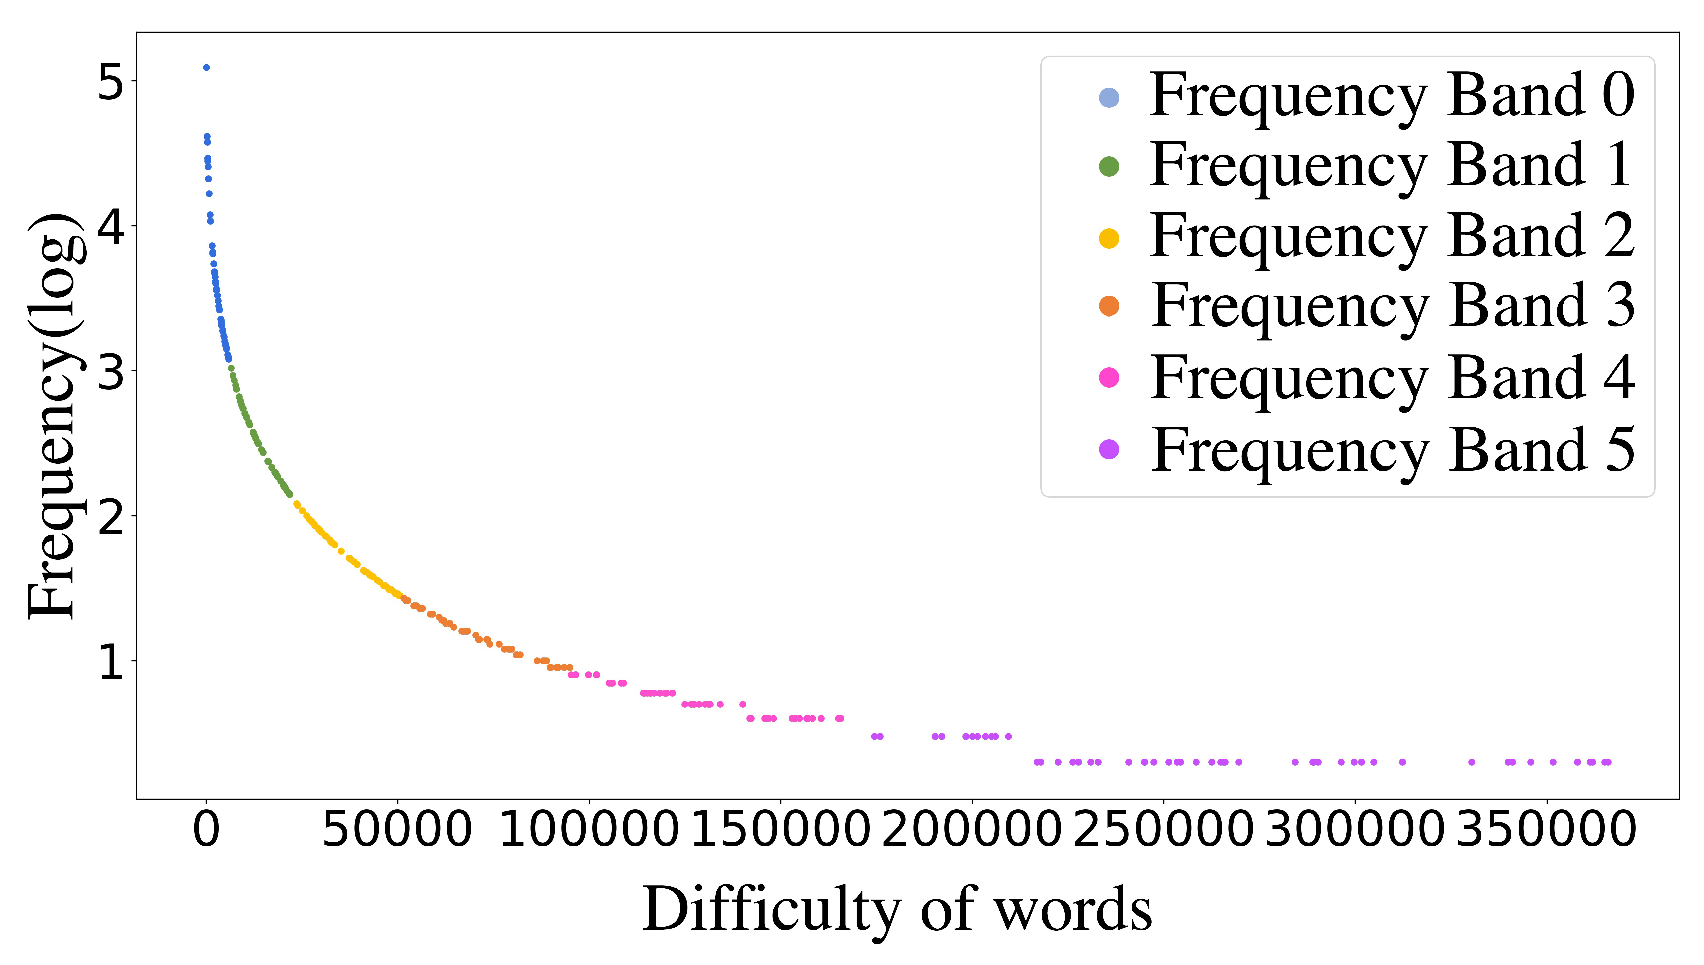
\epsfig{file=figure/cluster.eps,width=.8\columnwidth}
\vspace*{-4ex}
\caption{Numbers of Clusters vs. Number of Matching Frames in FrameNet}
\label{fig:cluster}
\end{figure}




